\providecommand{\main}{../main}
\documentclass[\main/main.tex]{subfiles}
\graphicspath{{../images/}}
\begin{document}
\section{
    動径量子化
}
%------------------------------------------------%
演算子形式の場の理論では、時間一定の超平面で時空をスライスし、その断面にHilbert空間を対応づける。
しかし、時空の切り方は一つではない。
回転対称な理論では時間の方向の取り方は任意であるし、時空を曲面で切ることもできる。
好き勝手な切り方では良い性質は期待できないが、共形場理論におけるうまい切断面として、超球面がある。
このようにして得られる動径量子化は状態・演算子対応や演算子積展開といった共形場理論における強力な道具と密接に関係しているので、以降で詳しく見ていくことにする。

\subsection{
    動径量子化
}
時空上に特別な原点を1つ定め、座標を原点からの距離$r$と方向を表す単位ベクトル$𝒏$によって表すことにする。
$r$を固定し、角度方向に依存する場$ϕ(r,𝒏) = φ(𝒏)$を考え、ありうる全ての場をそれぞれHilbert空間の基底$|φ⟩$に対応づける。
    % 状態の規格化は
    % \begin{align}
    %     ∫\𝒟φ |φ⟩⟨φ| = 1
    %     \label{radial normalization}
    % \end{align}
    % と定める。
また時間発展演算子を
\begin{align}
    ⟨φ_\rm{f}|\^U(r_\rm{f},r_\rm{i})|φ_\rm{i}⟩
    ≔ ∫^{ϕ(r_\rm{f})=φ_\rm{f}}
        _{ϕ(r_\rm{i})=φ_\rm{i}}
        \𝒟ϕ \e^{-S[ϕ]}
    \label{radial evolution}
\end{align}
と定義する。
このような演算子形式を\textbf{動径量子化(radial quantization)}と呼ぶ。

\subsection{
    真空状態
}
動径量子化において、単位球面上の真空状態$|0⟩$は
\begin{align}
    ⟨φ|0⟩ = \f{1}{\√Z} ∫^{ϕ(r=1)=φ}_{r=0}\𝒟ϕ\e^{-S[ϕ]}
\end{align}
と定義される。一方$⟨0|$は
\begin{align}
    ⟨0|φ⟩ = \f{1}{\√Z} ∫^{r=∞}_{ϕ(r=1)=φ}\𝒟ϕ\e^{-S[ϕ]}
\end{align}
と定義される。
$\√Z$は規格化定数であり、作用に定数を足すことで無視できる。
\begin{figure}[H]
    \centering
    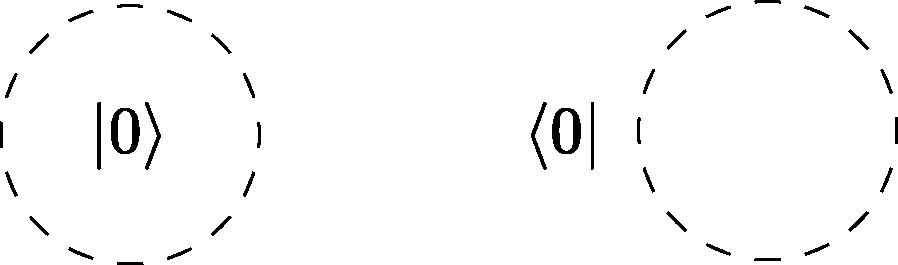
\includegraphics[width=0.5\hsize]{radial vacuum.pdf}
    \caption{動径量子化における真空状態}
\end{figure}
共形場理論では、トポロジカル演算子の性質から
\begin{align}
    \^P_μ|0⟩ = \^M_{μν}|0⟩ = \^D|0⟩ = \^K_μ|0⟩ = 0
    \label{vacuum symmetry}
\end{align}
が成り立つ。同様に
\begin{align}
    ⟨0|\^P_μ = ⟨0|\^M_{μν} = ⟨0|\^D = ⟨0|\^K_μ = 0
\end{align}
が成り立つ。
これは以下のように図示できる。
\begin{figure}[H]
    \centering
    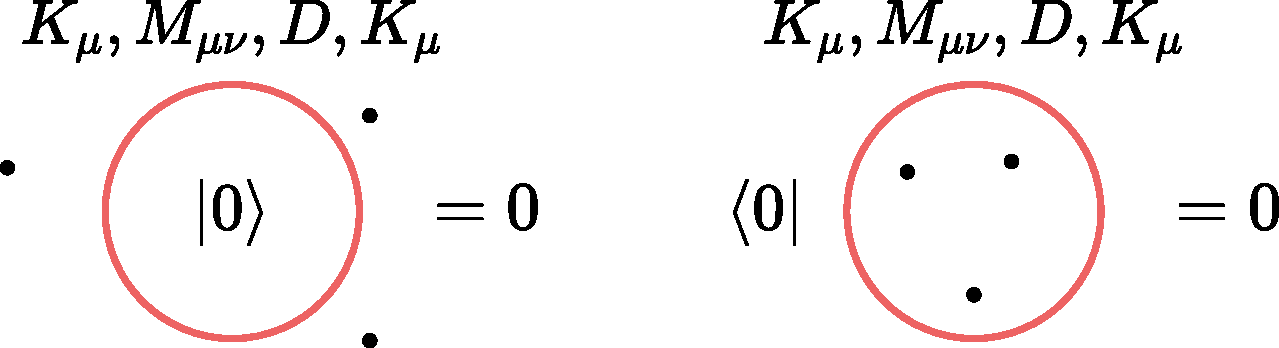
\includegraphics[width=0.6\hsize]{../images/symmetry_of_vacuum.pdf}
    \caption{真空の対称性}
\end{figure}
一つ目の式はトポロジカル演算子を1点に収縮できることから明らかである。
また二つ目の式は期待値に含まれる全ての演算子を一斉に座標変換しても相関関数が変わらないことから分かる。

\subsection{
    シリンダー時空
}
動径量子化では$r$ごとに動径一定面(超球面)の大きさが異なるため、$r$の異なるHilbert空間の次元が等しくならず、同一視できないという問題が発生する。
例えば格子正則化した場合を考えると、$r ≤ |x| ≤ r+δr$となるような格子点の数は$r$によって異なるので、転送行列を作ろうとすると正方行列ではなくなってしまう。
これを正方行列にしたいならば、$r$ごとに自由度を適当に積分して間引いてやらないといけない。

そのために、$τ =\log r$として、$(τ,𝒏)$で表されるシリンダー時空に移ることにする。
線素を$τ$を使って表すと、
\begin{align}
    \d{s}²_{ℝ^d} = \d{r}² + r²\d{s²}_{S^{d-1}}
    = \e^{2τ}(\dτ²+\d{s²}_{S^{d-1}})
    = \e^{2τ}\d{s}²_{ℝ×S^{d-1}}
\end{align}
となるので、Euclid空間$ℝ^d$からシリンダー時空$ℝ×S^{d-1}$への変換は共形変換になっている。
% \footnote{
% 正確には$ℝ^d$から原点を除いた空間がシリンダー時空に対応する。
% }
ここで$\d{s²}_{S^{d-1}}$は極座標の線素を表す。
\begin{figure}[H]
    \centering
    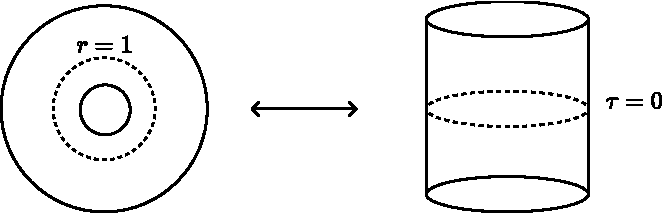
\includegraphics[width=0.5\hsize]{../images/cylinder spacetime.pdf}
    \caption{シリンダー時空}
\end{figure}
Euclid空間の経路積分からシリンダー時空の経路積分に移ることで、動径ごとの自由度の数が揃えられるため、性質の良い演算子形式が期待できる。
ただし、そのためには場所ごとに倍率の異なるくりこみ変換を行う必要があり、したがって共形不変性が必要なことに注意する。

理論のスケール不変性から
\begin{align}
    \⟨𝒪_1(x_1)⋯𝒪_N(x_N)\⟩
    = \f{1}{r_1^{Δ_1}}⋯\f{1}{r_N^{Δ_N}}
    f(\{n_i\},\{τ_i-τ_j\})
\end{align}
と表せるので、シリンダー時空上で定義される場$𝒪_\rm{cyl.}(τ,𝒏)$を、
\begin{align}
    𝒪_\rm{cyl.}(τ,𝒏) = r^Δ𝒪(x) = \e^{Δτ} 𝒪(x)
\end{align}
とする。
シリンダー時空への変換では局所的には$x → x/r$というくりこみ変換をしているので、このように場を定義しなおすのは妥当である。
すると相関関数は
\begin{align}
    \⟨𝒪_1(x_1)⋯𝒪_n(x_n)\⟩
    =\f{1}{r_1^{Δ_1}}⋯\f{1}{r_N^{Δ_N}}\⟨𝒪^\rm{cyl.}_1(x_1)⋯𝒪^\rm{cyl.}_n(x_n)\⟩
\end{align}
となる。したがって、シリンダー時空の相関関数はEuclid空間の相関関数を無次元化したものになっている。

\subsection{
    シリンダー時空の演算子形式
}
シリンダー時空では素朴に定義される(\ref{radial evolution})は修正を受ける。
まず、$τ$を固定して超球面上の場$ϕ_\rm{cyl}.(τ,𝒏) = φ(𝒏)$を考え、これを$|φ⟩$に対応づける。
ここで、$ϕ_\rm{cyl.}(τ,𝒏) = \e^{Δ_ϕτ}ϕ(x)$である。
シリンダー時空における時間発展演算子は
\begin{align}
    ⟨φ_\rm{f}|\^U(τ_\rm{f},τ_\rm{i})|φ_\rm{i}⟩
    ≔ ∫^{ϕ_\rm{cyl.}(τ_\rm{f})=φ_\rm{f}}
        _{ϕ_\rm{cyl.}(τ_\rm{i})=φ_\rm{i}}
        \𝒟ϕ \e^{-S[ϕ]}
\end{align}
と定義される。
境界条件はシリンダー時空の場$ϕ_\rm{cyl.}(τ,𝒏)=\e^{Δ_ϕτ}ϕ(x)$に対して課されていることに注意する。
規格化条件
\begin{align}
    ∫\𝒟φ|φ⟩⟨φ| = 1
\end{align}
を課すことで時間発展演算子の加法性
\begin{align}
    \^U(τ_1,τ_3) = \^U(τ_1,τ_2)\^U(τ_2,τ_3)
\end{align}
が分かる。
場$𝒪(τ,𝒏)$の質量次元が$Δ$であるとき、期待値は
\begin{align}
    \⟨𝒪_\rm{cyl.}(τ,𝒏)\⟩
    &
    = \e^{Δτ}∫\𝒟φ ⟨0|φ⟩𝒪[\e^{-Δ_ϕτ}φ(𝒏)]⟨φ|0⟩
    \∅ &
    = ∫\𝒟φ ⟨0|φ⟩𝒪[φ(𝒏)]⟨φ|0⟩
    \∅ &
    = ⟨0|\^U(0,τ)\^𝒪(𝒏)\^U(τ,0)|0⟩
\end{align}
となる。
したがって、$𝒪_\rm{cyl.}(τ,𝒏)=\e^{Δτ}𝒪(x)$はHeisenberg表示
\begin{align}
    \^𝒪(τ,𝒏) = \^U(0,τ)\^𝒪(𝒏)\^U(τ,0)
    \label{radial Heisenberg picture}
\end{align}
に対応することが分かる。
以降の議論でハットのついた演算子は全て無次元化されており、$\^𝒪(τ,𝒏)$は$𝒪(τ,𝒏)$ではなく$𝒪_\rm{cyl.}(τ,𝒏)$に対応するので注意してほしい。
% $N$点関数は動径順序積(原点に近い方を右に並べる)を用いて、
% \begin{align}
%     \e^{(Δ_1+⋯+Δ_N)τ}\⟨𝒪_1(x_1)⋯𝒪_N(x_N)\⟩
%     = ⟨0|𝖱^*[\^𝒪_1(x_1)⋯\^𝒪_N(x_N)]|0⟩
% \end{align}
% と書ける。

ここで、Ward-Takahashi恒等式から
\begin{align}
    𝒪_\rm{cyl.}(τ,𝒏)
    = \e^{Δτ}\e^{τ\∂*{τ}}𝒪(0,𝒏)
    = \e^{τD}𝒪(0,𝒏)
\end{align}
が成り立つので、
\begin{align}
    \^𝒪(τ,𝒏) = \e^{τ\^D}\^𝒪(0,𝒏)\e^{-τ\^D}
    \label{scale Ward-Takahashi identity}
\end{align}
となる。ただし、$\^D$は
\begin{align}
    \^D = -∫\dΩ n_μ n^ν\^T^μ{}_ν
\end{align}
と定義される。
$\dΩ$は極座標の測度であり、$n_μ = x_μ/r$である。
(\ref{radial Heisenberg picture})と
(\ref{scale Ward-Takahashi identity})を比較して、
\begin{align}\tcboxmath{
    \dv{τ}\^U(τ,0) = -\^D
}\end{align}
が得られる。
したがって$\^D$は動径量子化においてHamiltonianの役割をもつ。

\subsection{
    状態・演算子対応
}
スケール不変性をもつ場の理論では、$d-1$次元球面上で定義された状態と、その中心にある局所演算子が1対1対応するという良い性質がある。
これを以下で示すが、議論は次の図にまとめられる。
\begin{figure}[H]
    \centering
    
\includegraphics[width=0.7\hsize]{state-operator.pdf}
    \caption{状態・演算子対応}
\end{figure}

まず、状態から対応する局所演算子を構成する。
演算子は任意の境界条件に対して相関関数が計算できれば定義できる。
$D$の固有値$Δ$の固有状態$|𝒪⟩$が$τ=0$で定義されているとする。
もし$τ_1 > 0$に演算子$𝒪_1$が挿入された場合、相関関数は
\begin{align}
    \⟨𝒪_1(x_1)𝒪(0)\⟩
    &
    ≔ ⟨0|\^𝒪_1(τ_1,𝒏_1)|𝒪⟩
    = ∫\𝒟φ⟨φ|𝒪⟩ ∫^{τ=∞}_{ϕ_\rm{cyl.}(0)=φ}\𝒟ϕ
    𝒪_1(τ_1,𝒏_1)\e^{-S[ϕ]}
\end{align}
と計算できる。
一方この式で$τ_1 < 0$としようとしても、経路積分は$τ < 0$の領域を含まないため、うまく定義できない。
しかし、
\begin{align}
    |𝒪⟩ = \^U(0,τ)\^U(τ,0)|𝒪⟩
    = \e^{-Δτ}\^U(0,τ)|𝒪⟩
    = \e^{-Δτ}|𝒪(τ)⟩
\end{align}
と変形し、$τ → -∞$とすることで$τ < 0$にも演算子を挿入できる。
したがって、$|𝒪⟩$に対応する演算子$𝒪(0)$は
\begin{align}\tcboxmath{
    ⟨⋯𝒪(0)⟩ =\lim_{τ→-∞}\e^{-Δτ}⟨0|⋯|𝒪(τ)⟩
}\end{align}
によって定義される。

一般の$𝒪(x)$については$x$を原点とする動径量子化を考えて同様に定義できる。
% また
% \begin{align}
%     𝒪(x) = \e^{x⋅𝒫}𝒪(0)
% \end{align}
% によって定義することもできる。
状態の積も以下のように問題なく定義できる。
\begin{figure}[H]
    \centering
    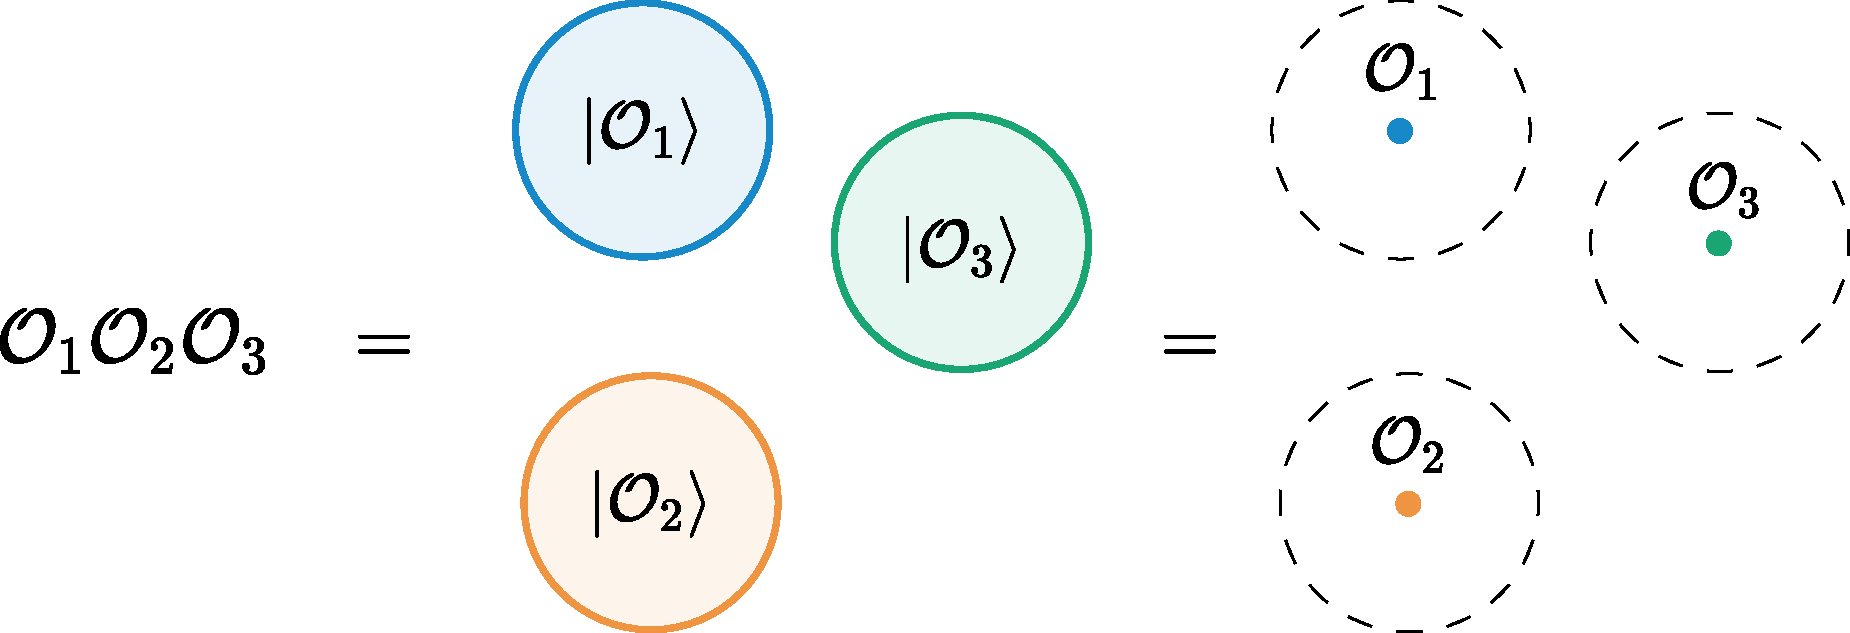
\includegraphics[width=0.7\hsize]{../images/state_to_operator.pdf}
    \caption{状態 ⇒ 演算子}
\end{figure}
スケール不変性がない場合はそれぞれの状態を重ねることができず、状態は剛体のような演算子として振る舞う。
スケール不変性があると、境界をいくらでも縮めることができるので、状態を局所演算子に対応づけられる。

次に、局所演算子から対応する状態を構成する。
演算子$𝒪(x=0)$に対し、状態$|𝒪⟩$は$r < 1$での経路積分を行った後の境界として得られる。
すなわち、
\begin{align}\tcboxmath{
    ⟨φ|𝒪⟩ =  ∫^{ϕ(τ=0)=φ}_{τ=-∞}𝒪(x=0)\e^{-S[ϕ]}
}\end{align}
と定義する。
$𝒪(x)$に対応する状態は$x$を中心とする動径量子化で同様に構成することができる。
% あるいは、
% \begin{align}
%     |𝒪(x)⟩ = \e^{n⋅\^P}\^𝒪(x)\e^{-n⋅\^P}|0⟩
%     = \e^{n⋅\^P}|𝒪⟩
% \end{align}
% によって定義できる。ここで$\^P_μ|0⟩=0$を用いた。

状態・演算子対応によって、プライマリー場に対応するプライマリー状態を構成することができる。
プライマリー場は
\begin{align}
    K_μ𝒪(0) = 0,\␣
    M_{μν}𝒪(0) = -𝒮_{μν}𝒪(0),\␣
    D𝒪(0) = Δ𝒪(0)
\end{align}
を満たすので、これに対応する状態$|𝒪⟩$は
\begin{align}
    \^K_μ|𝒪⟩ = 0,
    \␣
    \^M_{μν}|𝒪⟩ = -𝒮_{μν}|𝒪⟩,
    \␣
    \^D|𝒪⟩ = Δ|𝒪⟩
\end{align}
を満たす。
またディセンダント演算子に対応するディセンダント状態は
\begin{align}
    \^P_μ|𝒪⟩,\^P_μ\^P_ν|𝒪⟩,…
\end{align}
のように構成される。
% \printbibliography
\end{document}